\chapter{Конструкторский раздел}
В этом разделе будет проведено проектирование базы данных и приложения. Будут приведены созданные таблицы, поля таблиц с указанием их семантического смысла. Будет представлена ER-модель созданной базы данных.Будет выбран тип приложения. Будут представлены схемы основных алгоритмов, необходимых для функционирования приложения.

\section{Проектирование базы данных}

База данных приложения будет реализована с помощью следующих таблиц:

\begin{enumerate}
	\item таблица продуктов Product
	\item таблица заказов Order
	\item таблица отзывов Review
	\item таблица оценок продуктов Likeproduct
	\item таблица оценок отзывов Likereview
	\item таблица категорий продуктов Category
	\item таблица профилей Profile
	\item таблица пользователей User
\end{enumerate}

Таблица \textbf{User} содержит информацию о пользователях приложения. Содержит следующие поля:

\begin{itemize}
	\item id --- первичный ключ, идентификатор пользователя;
	\item password --- пароль пользователя;
	\item username --- никнейм пользователя(логин);
	\item first\_name --- имя пользователя;
	\item last\_name --- фамилия пользователя;
	\item email --- электронная почта пользователя;
	\item is\_superuser --- логическое поле, обозначающее есть ли у пользователя все разрешения без их явного назначения;
	\item is\_staff --- логическое поле, обозначающее есть ли у пользователя доступ к сайту администратора;
	\item is\_active --- логическое поле, обозначающее активность записи;
	\item data\_joined --- дата и время создания учетной записи;
	\item last\_login --- дата и время последнего входа пользователя в систему.
\end{itemize}

Таблица \textbf{Profile} содержит информацию о профилях пользователей. Содержит следующие поля:

\begin{itemize}
	\item id --- первичный ключ, идентификатор профиля;
	\item user\_id --- внешний ключ, соответствует id пользователя приложения;
	\item birth\_date --- дата рождения;
	\item address --- адрес пользователя;
	\item sex --- пол пользователя;
	\item avatar --- путь до картинки с аватаром пользователя.
\end{itemize}

Таблица \textbf{Product} содержит информацию о товарах, доступных на сайте. Содержит следующие поля:

\begin{itemize}
	\item id --- первичный ключ, идентификатор товара;
	\item title --- название товара;
	\item content --- описание товара;
	\item count --- количество товара;
	\item cost --- цена за единицу товара;
	\item image\_path --- путь до изображения товара;
	\item pub\_date --- дата публикации товара;
	\item rating --- оценка товара;
	\item volume --- объем флакона.
\end{itemize}

Таблица \textbf{Order} содержит информацию о заказах пользователей. Содержит следующие поля:

\begin{itemize}
	\item id --- первичный ключ, идентификатор заказа;
	\item status --- статус заказа;
	\item comment --- комментарий к заказу;
	\item order\_date --- дата создания заказа;
	\item date\_of\_completion --- дата выполнения заказа;
	\item profile\_id --- внешний ключ, соответствует id профиля заказчика.
\end{itemize}

Таблица \textbf{Review} содержит информацию об отзывах на товары. Содержит следующие поля:

\begin{itemize}
	\item id --- первичный ключ, идентификатор отзыва;
	\item content --- описание товара;
	\item review\_date --- дата публикации отзыва;
	\item profile\_id --- внешний ключ, соответствует id профиля, оставившего отзыв;
	\item product\_id --- внешний ключ, соответствует id товара, на который оставили отзыв.
\end{itemize}

Таблица \textbf{Likeproduct} содержит информацию об оценках на товары. Содержит следующие поля:

\begin{itemize}
	\item id --- первичный ключ, идентификатор оценки на товар;
	\item mark --- оценка, оставленная пользователем;
	\item profile\_id --- внешний ключ, соответствует id профиля, оставившего оценку;
	\item product\_id --- внешний ключ, соответствует id товара, на который оставили оценку.
\end{itemize}

Таблица \textbf{Likereview} содержит информацию об оценках на отзывы. Содержит следующие поля:

\begin{itemize}
	\item id --- первичный ключ, идентификатор оценки на отзыв;
	\item mark --- оценка, оставленная пользователем;
	\item profile\_id --- внешний ключ, соответствует id профиля, оставившего оценку;
	\item review\_id --- внешний ключ, соответствует id отзыва, на который оставили оценку.
\end{itemize}

Таблица \textbf{Category} содержит информацию о категориях товаров. Содержит следующие поля:

\begin{itemize}
	\item id --- первичный ключ, идентификатор категории;
	\item name --- название категории.
\end{itemize}

Таблица \textbf{OrdersProducts} содержит информацию о связи между заказами и товарами, а также хранит количество данного товара в заказе. Содержит следующие поля:

\begin{itemize}
	\item id --- первичный ключ, идентификатор категории;
	\item order\_id --- внешний ключ, соответствует id заказа;
	\item product\_id --- внешний ключ, соответствует id продукта;
	\item cnt --- количество товара в заказе.
\end{itemize}

\newpage

На рисунке \ref{er_db} приведена инфологическая модель базы данных.

\captionsetup{singlelinecheck = false, justification=centering}
\begin{figure}[h!]
	\begin{center}
		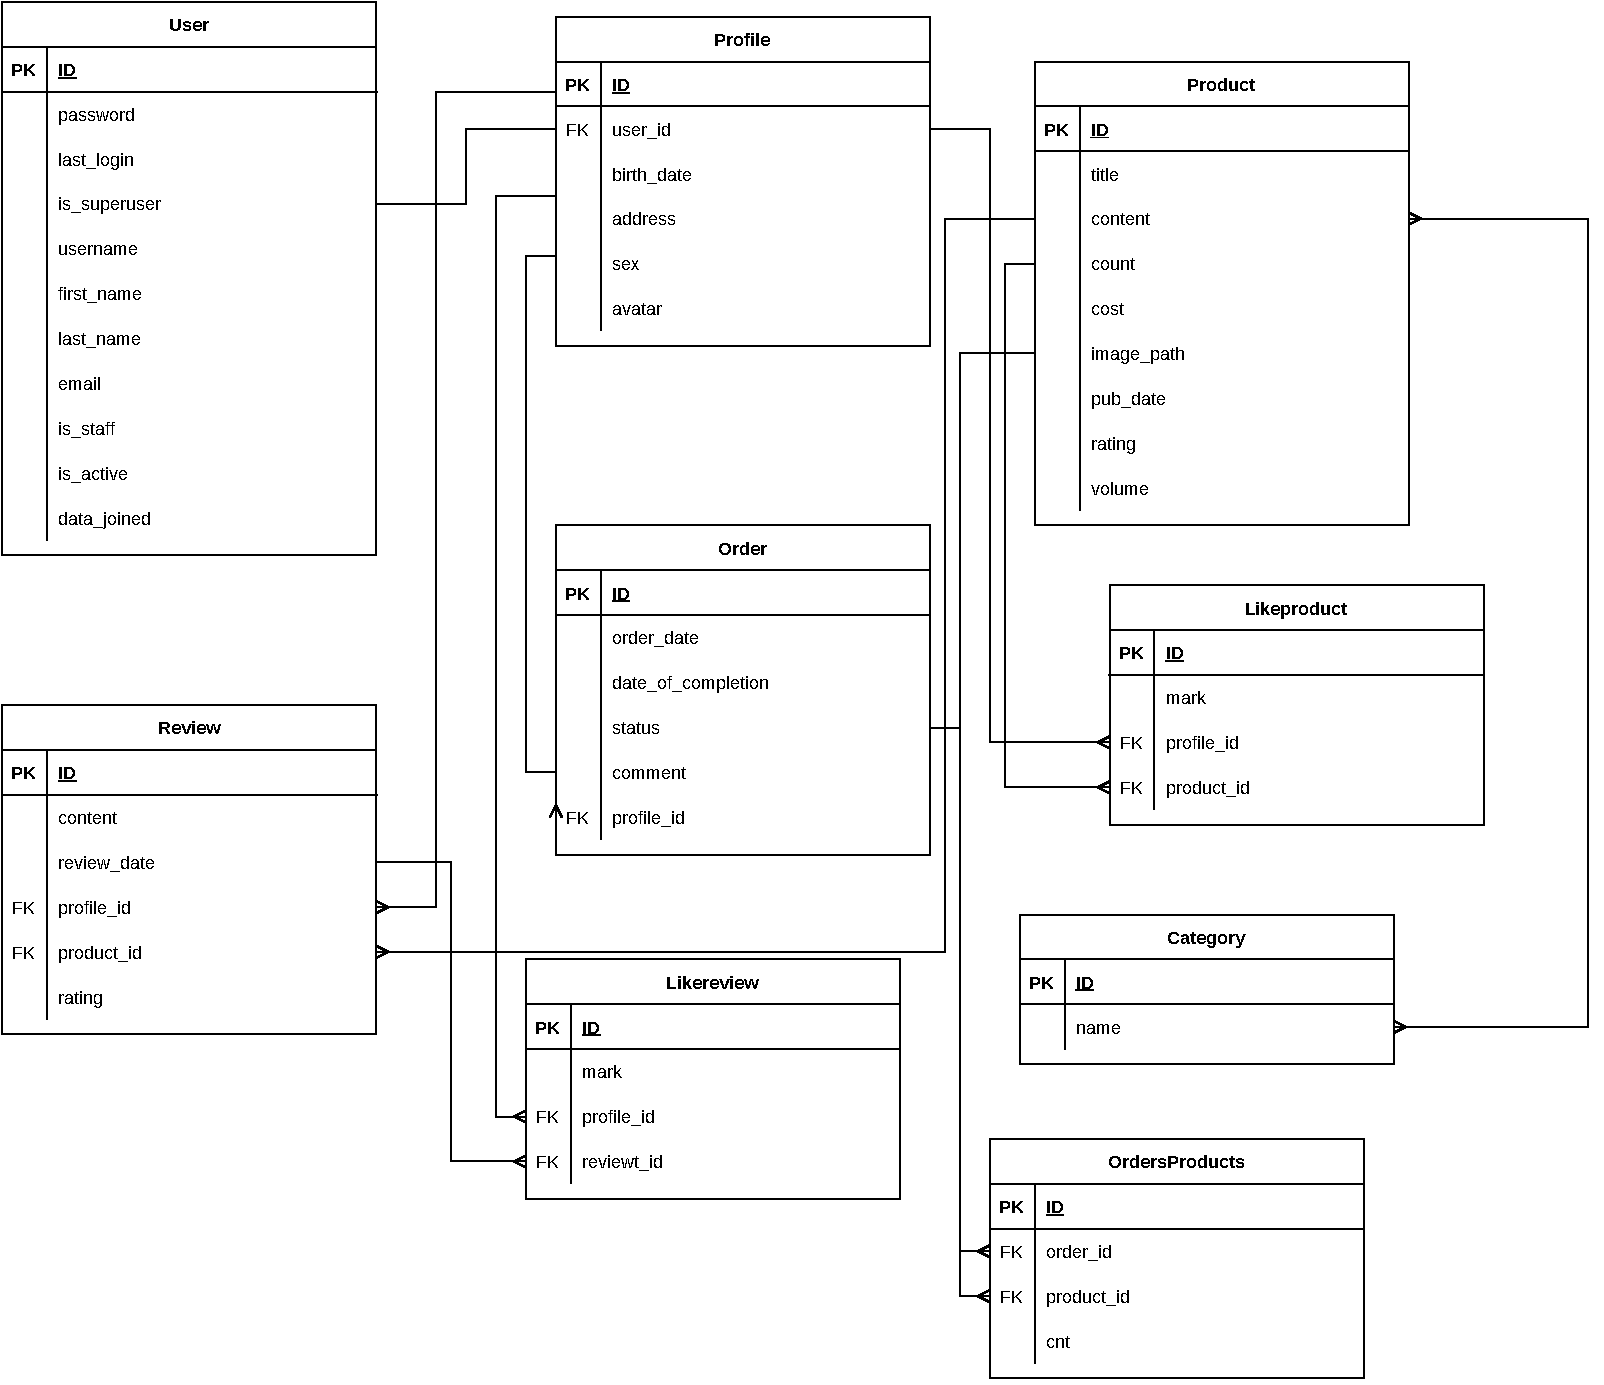
\includegraphics[scale=0.6]{assets/er_db.pdf}
	\end{center}
	\caption{Инфологическая модель базы данных}
	\label{er_db}
\end{figure}

\section{Схемы триггеров}

На рисунке \ref{decrease_count_trigger} приведена схема триггера, уменьшающего количество товара при заказе на количество единиц, заказанного товара.

\newpage

\captionsetup{singlelinecheck = false, justification=centering}
\begin{figure}[h!]
	\begin{center}
		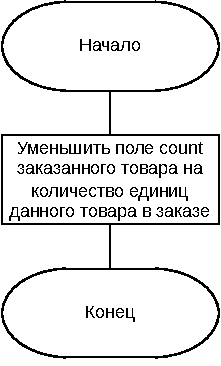
\includegraphics[scale=0.8]{assets/decrease_count_trigger.pdf}
	\end{center}
	\caption{Схема триггера decrease\_count}
	\label{decrease_count_trigger}
\end{figure}

На рисунке \ref{like_product_trigger} приведена схема триггера, изменяющего рейтинг товара при добавлении оценки на товар пользователем.

\captionsetup{singlelinecheck = false, justification=centering}
\begin{figure}[h!]
	\begin{center}
		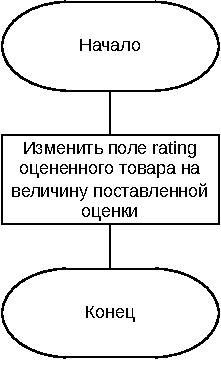
\includegraphics[scale=0.8]{assets/like_product_trigger.pdf}
	\end{center}
	\caption{Схема триггера like\_product\_insert}
	\label{like_product_trigger}
\end{figure}

На рисунке \ref{like_update_product_trigger} приведена схема триггера, изменяющего рейтинг товара на удвоенную оценку при изменеии оценки товара пользователем. 

\captionsetup{singlelinecheck = false, justification=centering}
\begin{figure}[h!]
	\begin{center}
		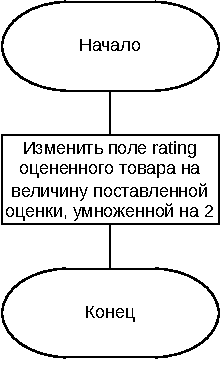
\includegraphics[scale=0.8]{assets/like_update_product_trigger.pdf}
	\end{center}
	\caption{Схема триггера like\_product\_update}
	\label{like_update_product_trigger}
\end{figure}
